\documentclass[border={1mm 1mm 1mm 1mm},tikz,10pt]{standalone}

\usetikzlibrary{shapes.geometric}

\usepackage{xcolor}
\definecolor{cnavy}{RGB}{4,41,112}
\definecolor{cgrey}{RGB}{72,72,72}
\definecolor{cred}{RGB}{192,0,0}
\definecolor{cgreen}{RGB}{0,157,0}

\begin{document}
	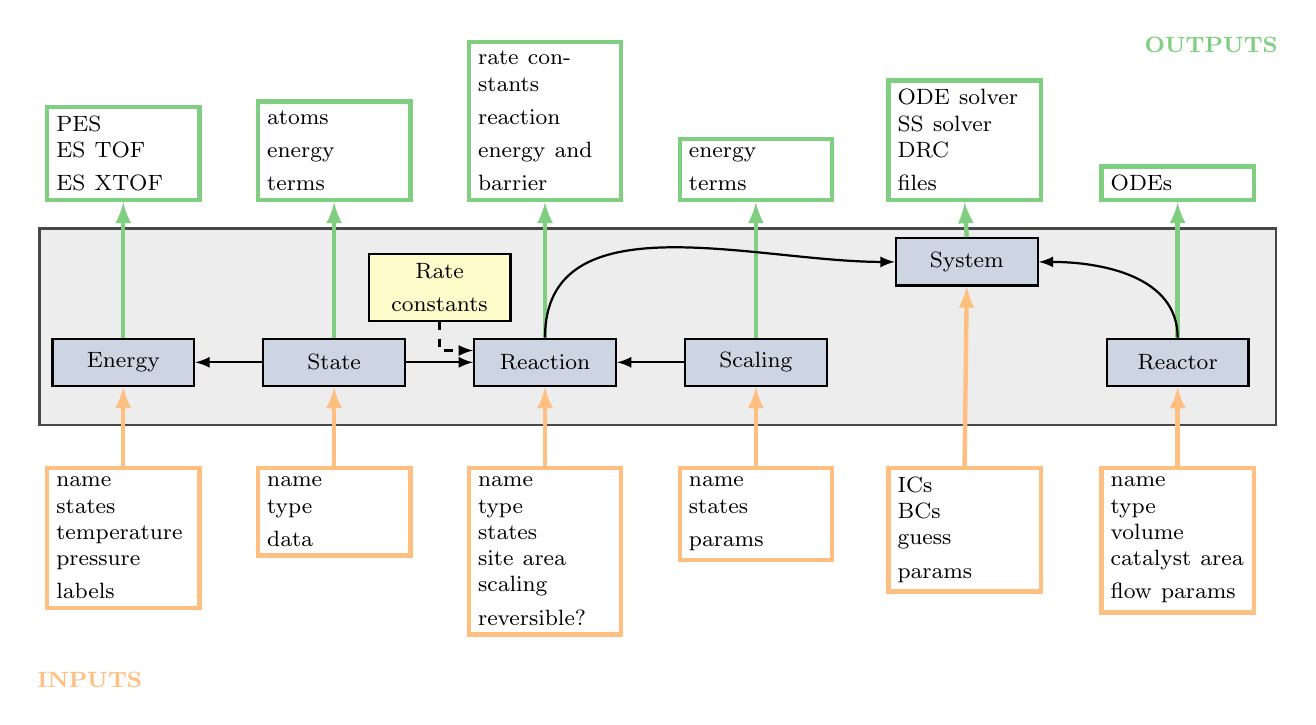
\begin{tikzpicture}[x=1cm, y=1cm, >=latex]
		\def\xleft{0}
		\def\xright{16}
		\def\ydown{0}
		\def\yup{8.5}
		\def\xmid{8}
		\def\ymid{4.25}
		\draw[draw=none, use as bounding box] (\xleft, \ydown) rectangle (\xright, \yup);
		\clip (\xleft-0.1, \ydown-0.1) rectangle (\xright+0.1, \yup+0.1);
		
		\def\rlen{1.8cm}
		\def\rwid{0.6cm}
		\def\blen{1.7cm}
		\def\rsep{0.85cm}
		\def\isep{1.cm}
		\def\rupp{1.5}
		\def\bmark{\textcolor{cgrey}{$\bullet$ }}
			
		\draw[fill=cgrey!10, draw=cgrey, thick] ([xshift=0.15cm, yshift=-0.8*\isep]\xleft, \ymid) rectangle ([xshift=-0.15cm, yshift=1.7*\isep]\xright, \ymid);
		
		% Boxes
		\node[anchor=west, fill=cnavy!20, draw=black, thick, minimum width=\rlen, minimum height=\rwid] (energy) at ([xshift=0.3cm]\xleft, \ymid)
			{\footnotesize{Energy}};
	
		\node[anchor=west, fill=cnavy!20, draw=black, thick, minimum width=\rlen, minimum height=\rwid] (state) at ([xshift=\rsep]energy.east)
			{\footnotesize{State}};	

		\node[anchor=west, fill=cnavy!20, draw=black, thick, minimum width=\rlen, minimum height=\rwid] (reaction) at ([xshift=\rsep]state.east)
			{\footnotesize{Reaction}};
		
		\node[anchor=west, fill=cnavy!20, draw=black, thick, minimum width=\rlen, minimum height=\rwid] (scaling) at ([xshift=\rsep]reaction.east)
			{\footnotesize{Scaling}};		
		
		\node[anchor=west, fill=cnavy!20, draw=black, thick, minimum width=\rlen, minimum height=\rwid] (system) at ([xshift=\rsep, yshift=\rupp*\rsep]scaling.east)
			{\footnotesize{System}};		
		
		\node[anchor=west, fill=cnavy!20, draw=black, thick, minimum width=\rlen, minimum height=\rwid] (reactor) at ([xshift=\rsep, yshift=-1*\rupp*\rsep]system.east)
			{\footnotesize{Reactor}};
				
%		\node[anchor=west, fill=cnavy!20, draw=black, thick, minimum width=\rlen, minimum height=\rwid] (uncertainty) at ([xshift=\rsep]energy.east)
%		{Uncertainty};
		
		% Inputs
		\node[anchor=south west] at (\xleft, \ydown)
			{\footnotesize{\textcolor{orange!50}{\textbf{INPUTS}}}};		
		\node[anchor=north, fill=white, draw=orange!50, ultra thick, text width=\blen] (Ein) at ([yshift=-1*\isep]energy.south)
			{
				\footnotesize{name\\states\\temperature\\pressure\\labels}
			};
		\node[anchor=north, fill=white, draw=orange!50, ultra thick, text width=\blen] (Sin) at ([yshift=-1*\isep]state.south)
			{
				\footnotesize{name\\type\\data}
			};
		\node[anchor=north, fill=white, draw=orange!50, ultra thick, text width=\blen] (Rin) at ([yshift=-1*\isep]reaction.south)
			{
				\footnotesize{name\\type\\states\\site area\\scaling\\reversible?}
			};
		\node[anchor=north, fill=white, draw=orange!50, ultra thick, text width=\blen] (Scin) at ([yshift=-1*\isep]scaling.south)
			{
				\footnotesize{name\\states\\params}
			};
		\node[anchor=north, fill=white, draw=orange!50, ultra thick, text width=\blen] (Syin) at ([yshift=-1*\isep, xshift=\rsep+\rlen]scaling.south)
			{
				\footnotesize{ICs\\BCs\\guess\\params}
			};
		\node[anchor=north, fill=white, draw=orange!50, ultra thick, text width=\blen] (Rein) at ([yshift=-1*\isep]reactor.south)
			{
				\footnotesize{name\\type\\volume\\catalyst area\\flow params}
			};	

		% Input arrows
		\draw[ultra thick, ->, orange!50] (Ein.north) -- (energy.south);
		\draw[ultra thick, ->, orange!50] (Sin.north) -- (state.south);
		\draw[ultra thick, ->, orange!50] (Rin.north) -- (reaction.south);
		\draw[ultra thick, ->, orange!50] (Scin.north) -- (scaling.south);
		\draw[ultra thick, ->, orange!50] (Syin.north) -- (system.south);
		\draw[ultra thick, ->, orange!50] (Rein.north) -- (reactor.south);
	
		\node[anchor=south, fill=yellow!20, draw=black, thick, minimum width=\rlen, minimum height=\rwid, text width=\rlen-0.25cm, align=center] (constants) at ([xshift=-0.5*\rsep, yshift=0.6*\rsep]reaction.west)
			{\footnotesize{Rate\\constants}};
		\draw[thick, ->, dashed] (constants.south) -- ([xshift=-0.5*\rsep, yshift=0.25*\rwid]reaction.west) -- ([yshift=0.25*\rwid]reaction.west);
		
		% Outputs
		\node[anchor=north east] at (\xright, \yup)
			{\footnotesize{\textcolor{cgreen!50}{\textbf{OUTPUTS}}}};

		\node[anchor=south, fill=white, draw=cgreen!50, ultra thick, text width=\blen] (Eout) at ([yshift=1.72*\isep]energy.north)
			{
				\footnotesize{PES\\ES TOF\\ES XTOF}
			};
		\node[anchor=south, fill=white, draw=cgreen!50, ultra thick, text width=\blen] (Sout) at ([yshift=1.72*\isep]state.north)
			{
				\footnotesize{atoms\\energy terms}
			};
		\node[anchor=south, fill=white, draw=cgreen!50, ultra thick, text width=\blen] (Rout) at ([yshift=1.72*\isep]reaction.north)
			{
				\footnotesize{rate constants\\reaction energy and barrier}
			};
		\node[anchor=south, fill=white, draw=cgreen!50, ultra thick, text width=\blen] (Scout) at ([yshift=1.72*\isep]scaling.north)
			{
				\footnotesize{energy terms}
			};
		\node[anchor=south, fill=white, draw=cgreen!50, ultra thick, text width=\blen] (Syout) at ([yshift=1.72*\isep, xshift=\rsep+\rlen]scaling.north)
			{
				\footnotesize{ODE solver\\SS solver\\DRC\\files}
			};
		\node[anchor=south, fill=white, draw=cgreen!50, ultra thick, text width=\blen] (Reout) at ([yshift=1.72*\isep]reactor.north)
			{
				\footnotesize{ODEs}
			};
		
		% Output arrows
		\draw[ultra thick, <-, cgreen!50] (Eout.south) -- (energy.north);
		\draw[ultra thick, <-, cgreen!50] (Sout.south) -- (state.north);
		\draw[ultra thick, <-, cgreen!50] (Rout.south) -- (reaction.north);
		\draw[ultra thick, <-, cgreen!50] (Scout.south) -- (scaling.north);
		\draw[ultra thick, <-, cgreen!50] (Syout.south) -- (system.north);
		\draw[ultra thick, <-, cgreen!50] (Reout.south) -- (reactor.north);	
	
		% Arrows
		\draw[thick, ->] (state.west) -- (energy.east);
		\draw[thick, ->] (state.east) -- (reaction.west);
		\draw[thick, ->] (scaling.west) -- (reaction.east);
		\path[thick, ->] (reaction.north) edge[out=90, in=180] node [left] {} (system.west);
		\path[thick, ->] (reactor.north) edge[out=90, in=360] node [left] {} (system.east);
		
	\end{tikzpicture}
\end{document}